%---------------------------------------------------------------------
%  Writeup of the improved search of Run II data for single top quark
%  production at DZero.
%  Started: Oct 2006
%  Authors: The Single Top Working Group
%---------------------------------------------------------------------
%
\appendix
\section*{Appendix 4 --- Neural Network $B$-Tagging}
\label{appendix-nn-btagging}

We are using the neural network $b$-tagging algorithm version 1.1 from
the B-ID Agorithm Group. We present here an explanation of how we
apply this algorithm to Monte Carlo events. For data events, the
algorithm is applied directly.

\subsection{Taggability}
\label{taggability}

Taggability is defined as the probability that a jet is taggable,
where this means that a calorimeter jet is matched within $\Delta R <
0.5$ of a track jet, the track jet consists of at least two tracks,
with $\Delta R < 0.5$ between them, and the tracks used to form the
track jet have at least one SMT hit on them and at least one of the
tracks has $p_T > 1$~GeV.

Because our model of the detector does not completely match the real
one, we cannot apply the taggability requirements to Monte Carlo jets
directly and get the same answer as for data. We compensate for this
by instead applying taggability rate functions to the MC events.
These functions are parametrized in jet $\pt$, jet $\eta$ and primary
vertex $z$. They have been derived on the single top loose data
samples, where the isolation of the lepton is only required to be
loose (that is, all preselection except the tight lepton isolation) to
keep enough statistics for the measurement. Since these functions are
applied to tight samples, cross checks have been made to validate
their applicability. The observed taggability is measured (making the
jet selection for the jet to be taggable) on the tight data sample and
compared with the taggability rate function value in the same tight
data events. The results can be seen in
Fig.~\ref{fig:taggvalidation}. The observed taggability and the
predicted taggability give the same result within uncertainties.

\begin{figure}[!h!tbp]
\begin{center}
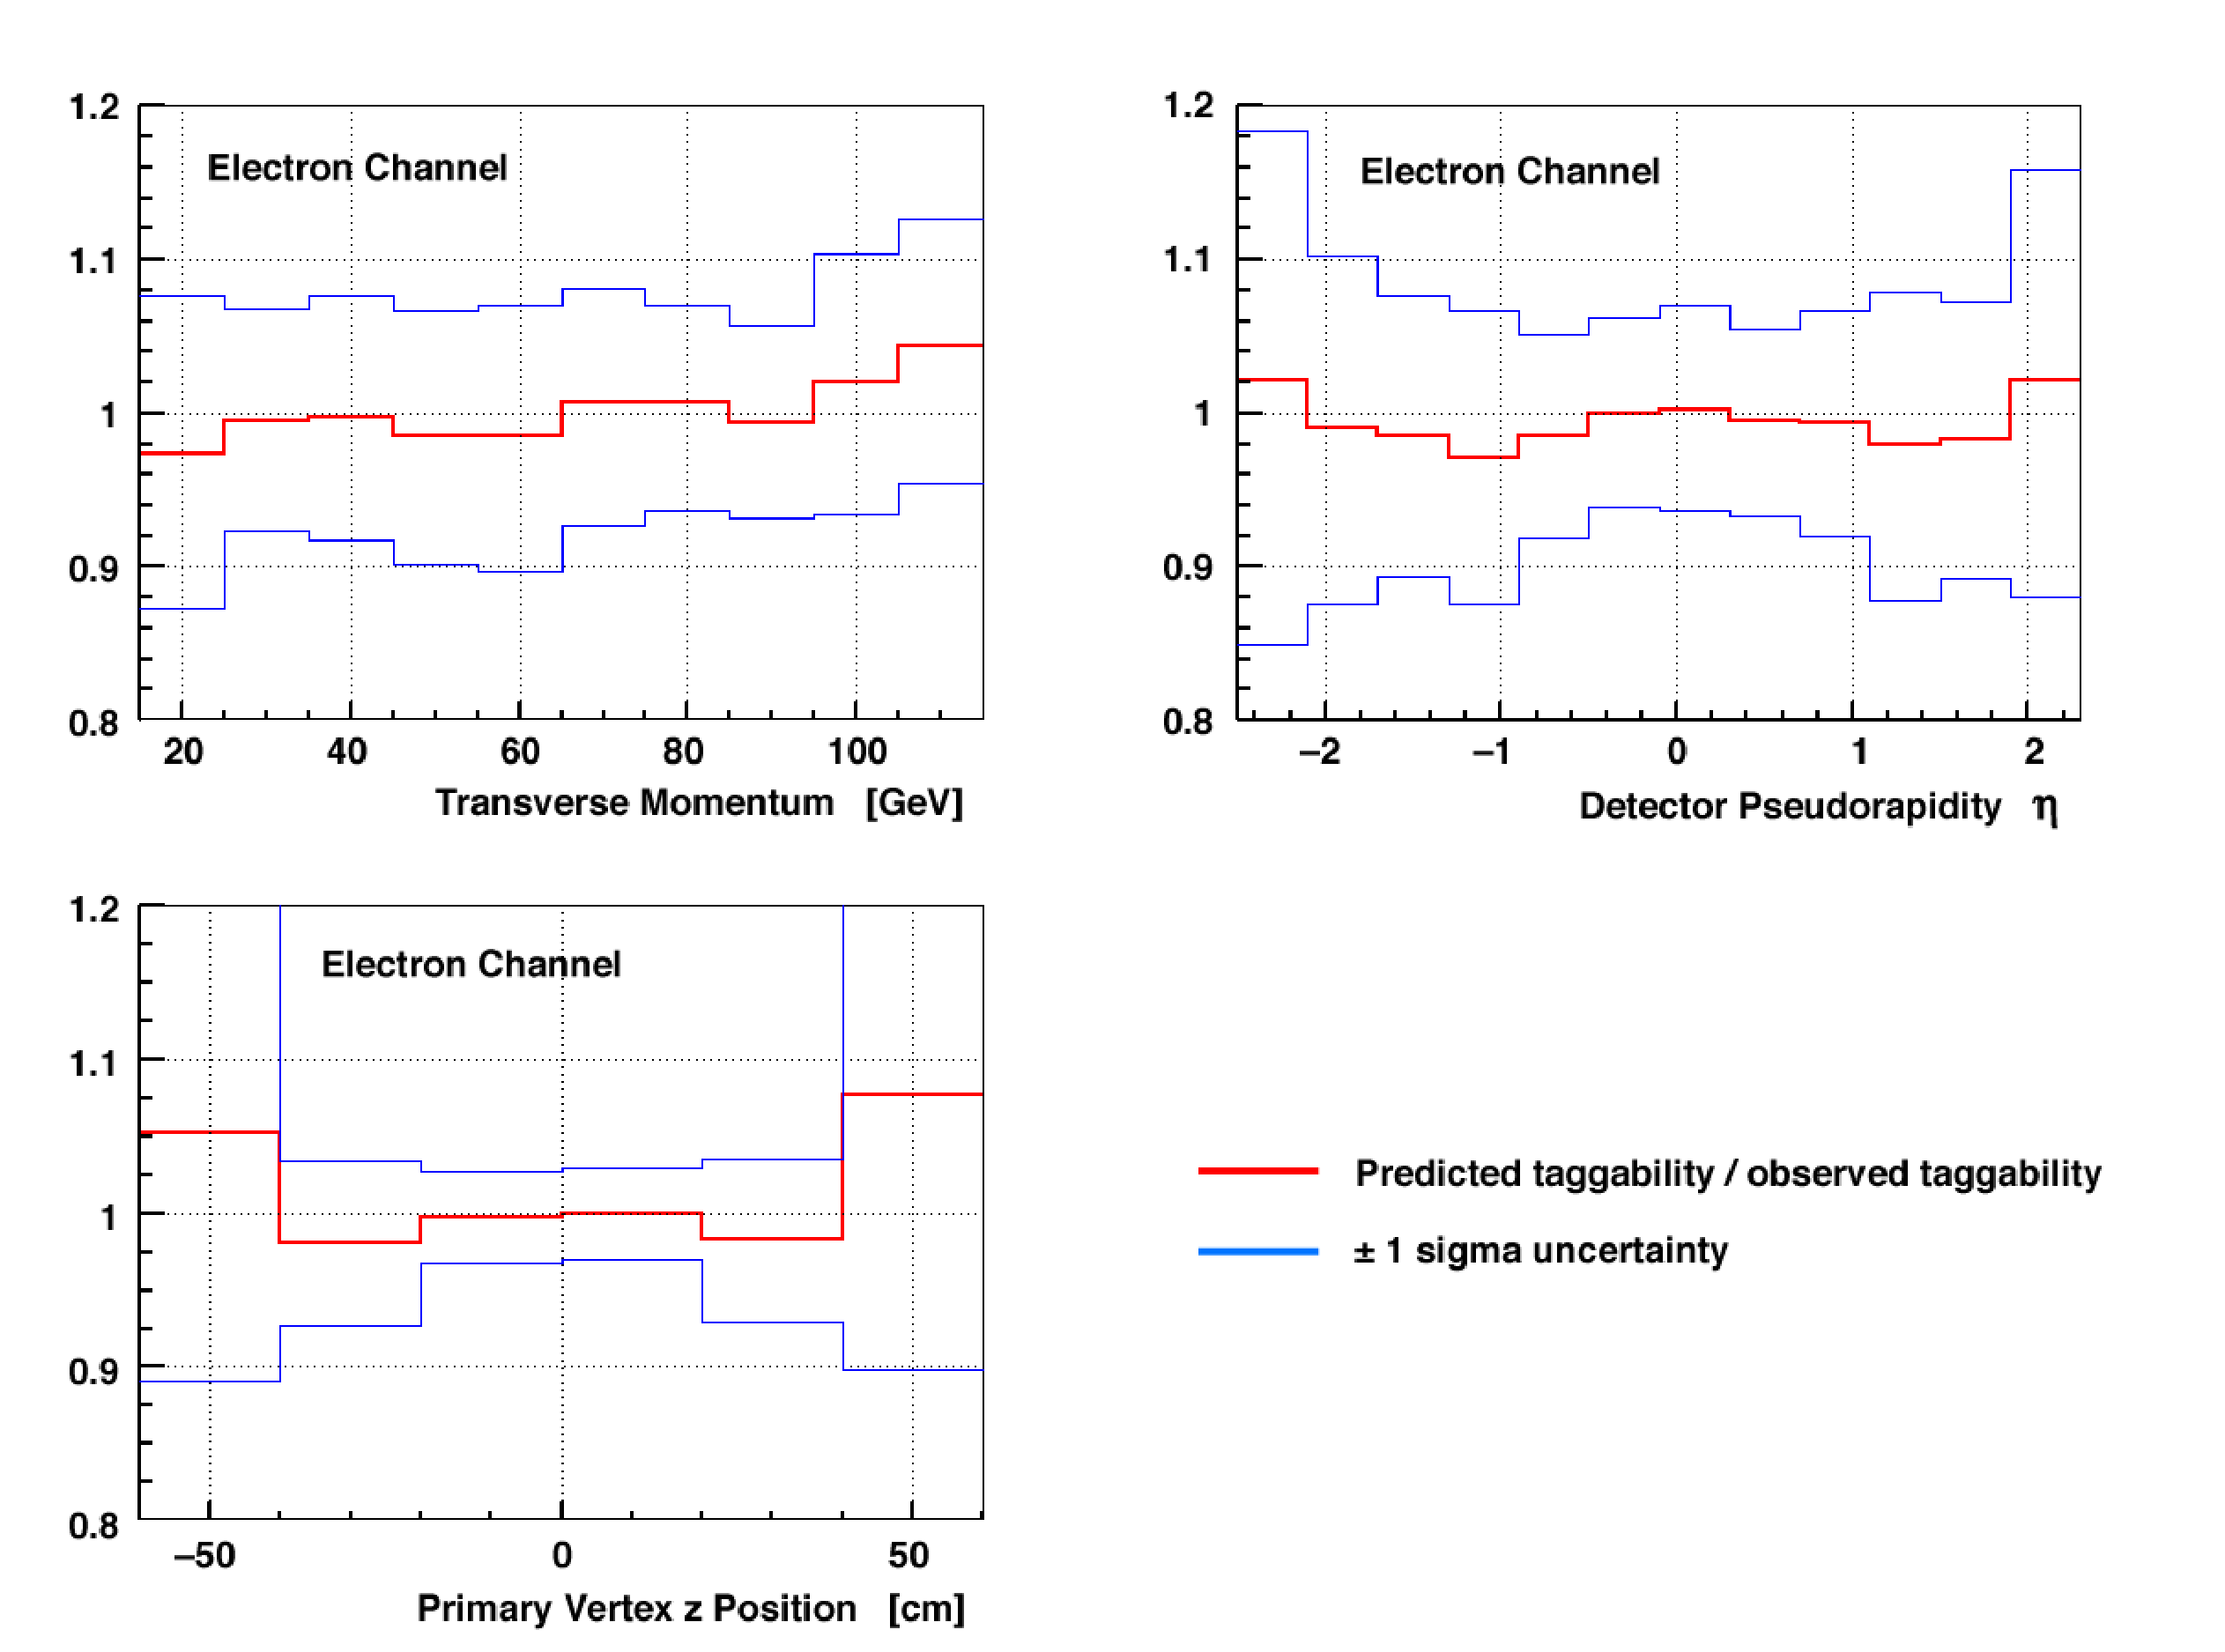
\includegraphics[width=0.49\textwidth]
{figures/taggability_el_validation.eps}
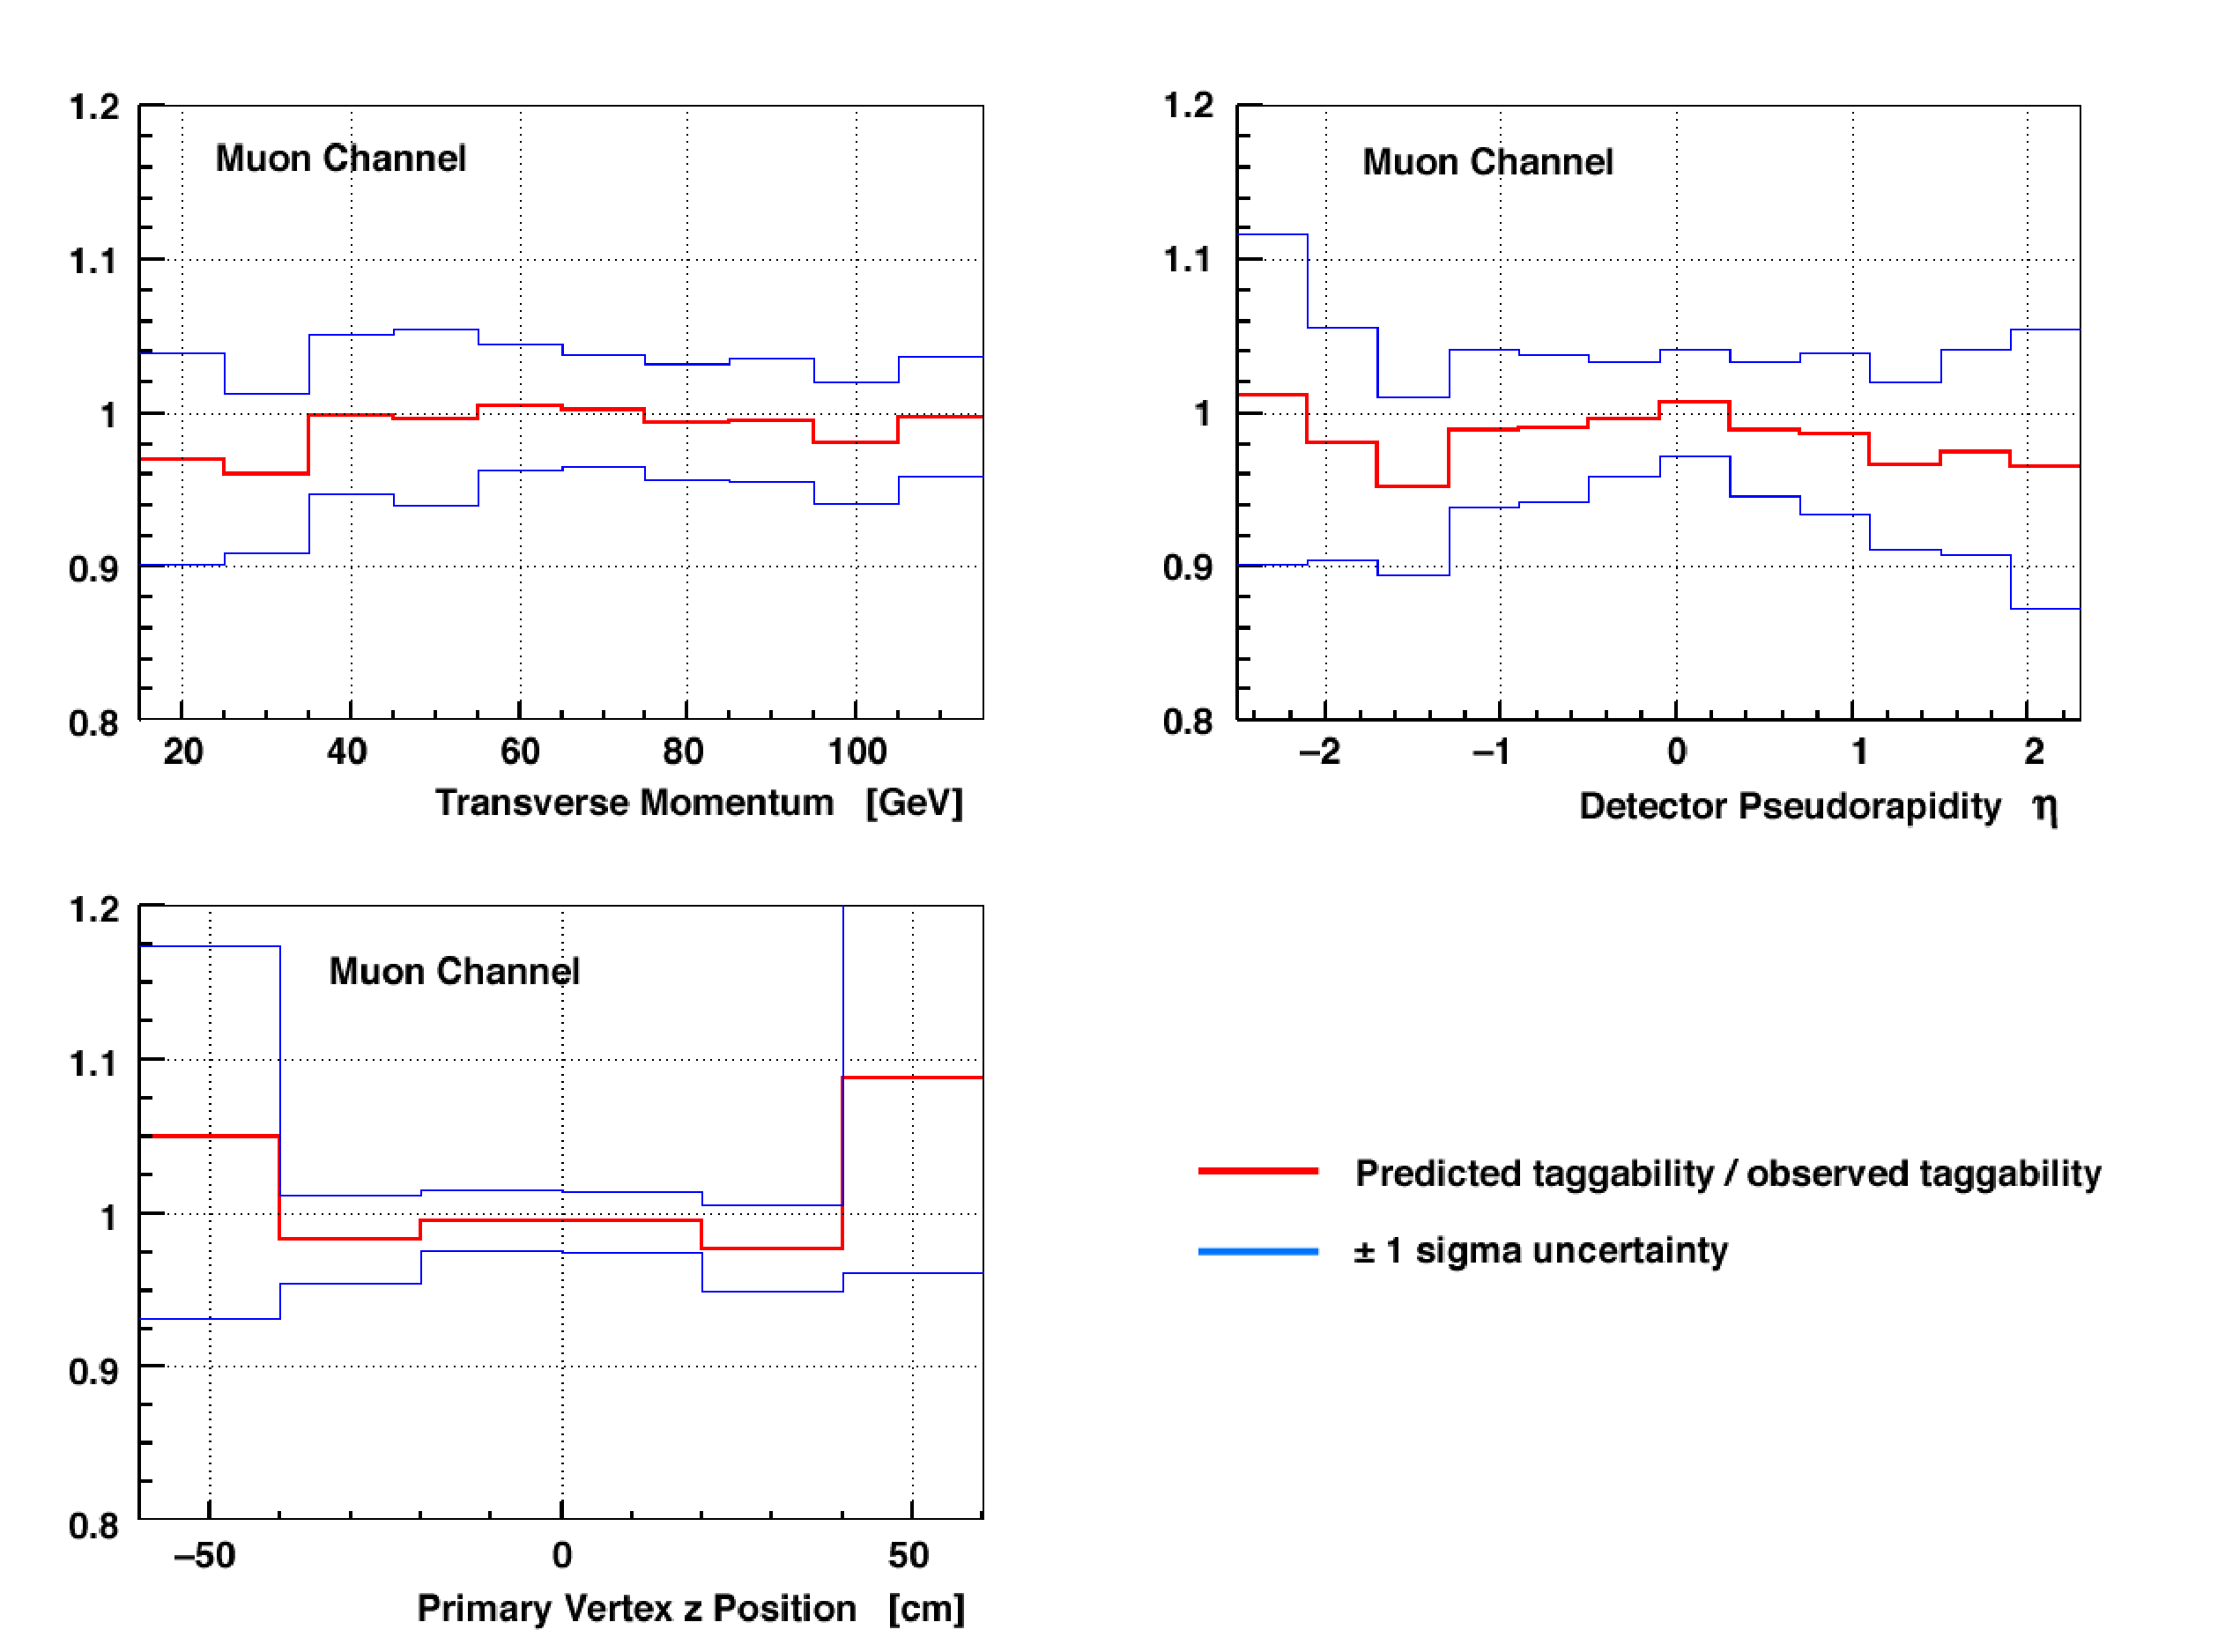
\includegraphics[width=0.49\textwidth]
{figures/taggability_mu_validation.eps}
\end{center}
\vspace{-0.1in}
\caption[tag]{The ratio of the predicted taggability rate function
over the observed taggability on the electron channel (upper plots)
and muon channel (lower plots) tight data sample. The taggability rate
function is derived on the loose data sample, but it matches the
observed taggability in the tight sample.}
\label{fig:taggvalidation}
\end{figure}

\clearpage

\subsection{$b$-Tagging Efficiencies}
\label{trfs}

The $b$-jet efficiency is measured in data, using a muon-in-jet sample
(BID sample) and a $b$-enriched subset consisting of muonic jets with
an away-jet tag probability of JLIP$<0.5$. This semileptonic
efficiency is denoted as $\varepsilon^{\rm DATA}_{b\to\mu}$. If we
apply the NN tagger to an MC sample with an admixture of $Z\to
b\bar{b}$ and $\ttbar$ MC, where the $b$~jets are forced to contain a
muon inside them, we obtain the semileptonic MC efficiency:
$\varepsilon^{MC}_{b\to\mu}$. The difference in efficiency between a
simulated jet and a jet in the data is parametrized in a data/MC scale
factor as a function of jet $\pt$ and $\eta$:
\vspace{-0.1in}
$$
SF_{b} = \frac{\varepsilon^{\rm DATA}_{b\to\mu}}
{\varepsilon^{MC}_{b\to\mu}}.
$$

To obtain the inclusive $b$-decay efficiency in data
$\varepsilon_{b}$, which is what we need to apply in our MC samples,
we just use:
\vspace{-0.1in}
$$
\varepsilon_b = \varepsilon^{\rm MC}_b \times SF_{b},
$$
\noindent where $\varepsilon^{\rm MC}_b$ is the efficiency to tag a
$b$~jet in an MC sample containing inclusive decays of the $b$~quark.
By using this procedure, we obtain the topological dependence of the
$b$-tagging efficiency from $\ttbar$ and $Z\to b\bar{b}$ samples,
while the overall efficiency normalization is calibrated to
data. However, one of our main backgrounds, $Wb\bar{b}$, produces
$b$~quarks not from $t$ or $Z$ decays, but from gluon splitting and
thus has somewhat different kinematics. It has been studied that
$b$~quarks from gluon splitting carry a smaller fraction of the total
jet momentum than $b$~quarks from $t$ or $Z$ decays. This results in a
5--10\% overestimation of the $\varepsilon_b$ over the tagger applied
directly to the MC, for jets below 30~GeV. The uncertainty on the
$\varepsilon_b$ is set large enough to cover this effect in this
region.
% See: http://www-d0.hef.kun.nl//askArchive.php?base=agenda&categ=a061800&id=a061800s1t1/transparencies

To obtain the inclusive $c$-quark $\varepsilon_c$, we assume that
$SF_c = SF_b$ and measure $\varepsilon^{\rm MC}_c$ in a combined MC
$c$ sample (with $Z$, QCD and $\ttbar$ decays to $c$ quarks). The
measured $\varepsilon_b$ and $\varepsilon_c$ dependences are shown in
Fig.~\ref{fig:NNTRFs} together with the direct tagger efficiency.

\vspace{0.1in}
\begin{figure}[!h!tbp]
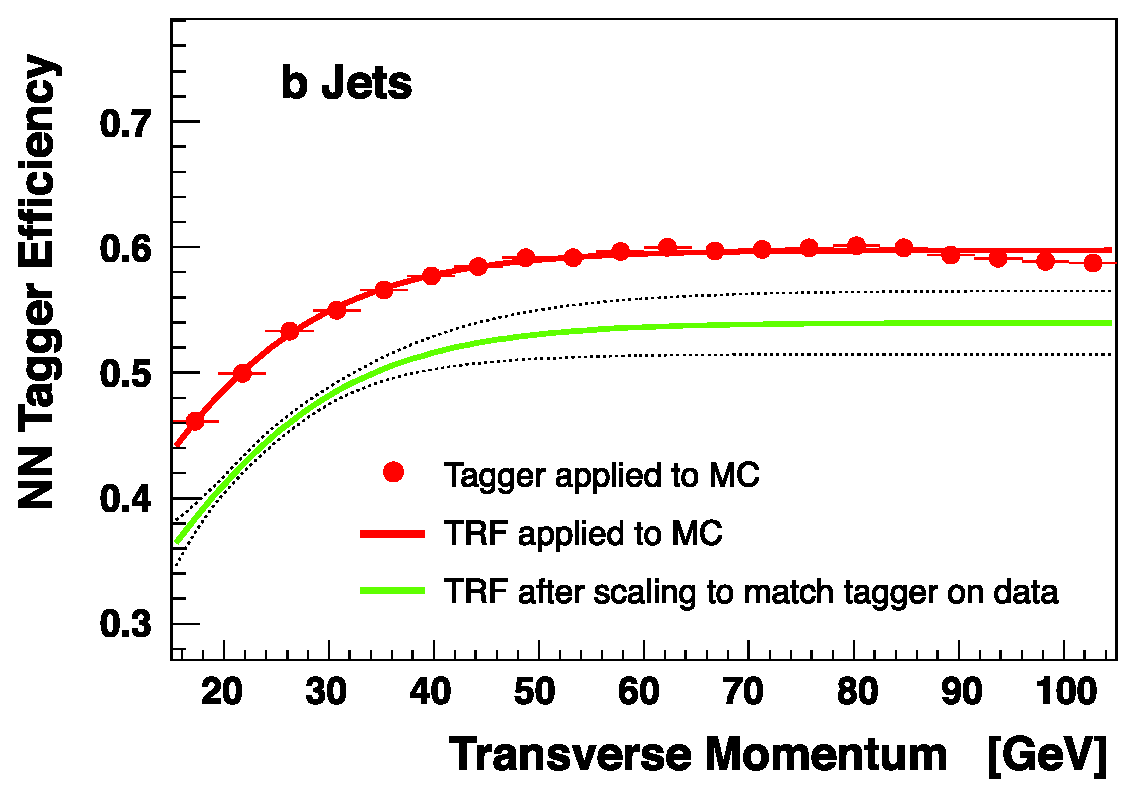
\includegraphics[width=0.32\textwidth]
{figures/TRF_b_pt.eps}
\hspace{0.5in}
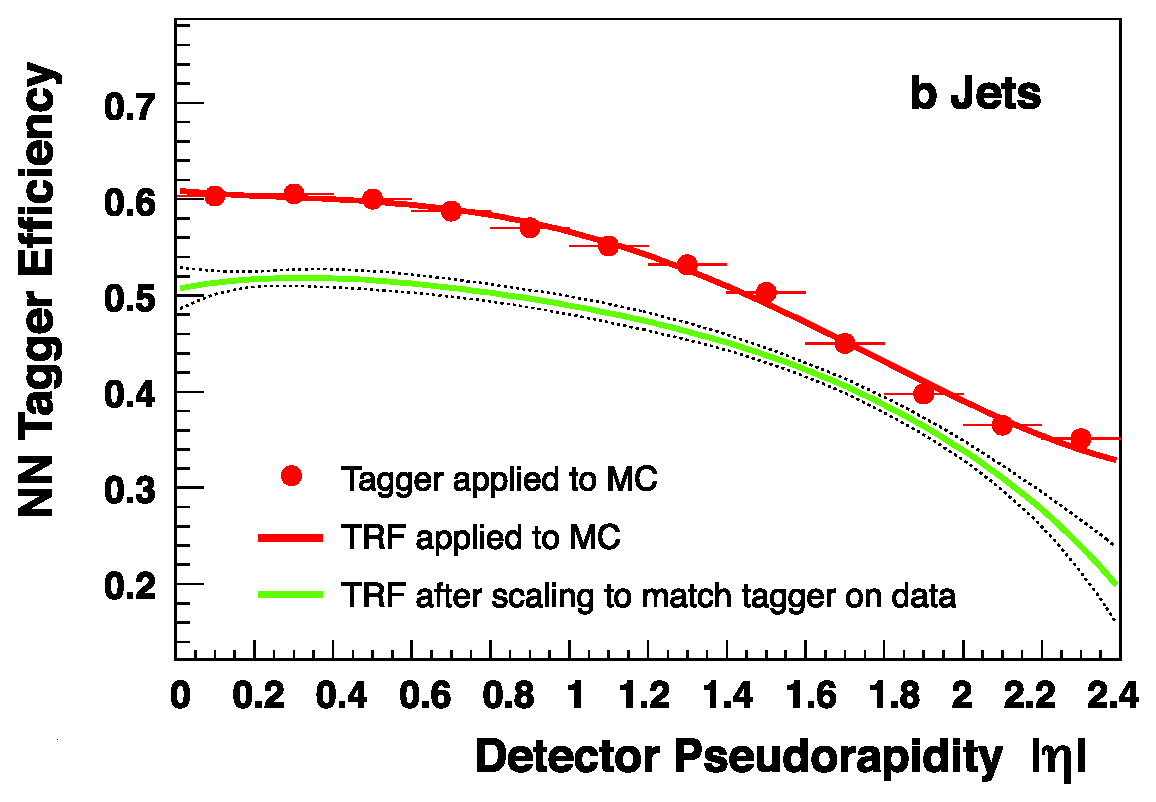
\includegraphics[width=0.32\textwidth]
{figures/TRF_b_eta.eps}
\hspace{0.1in}
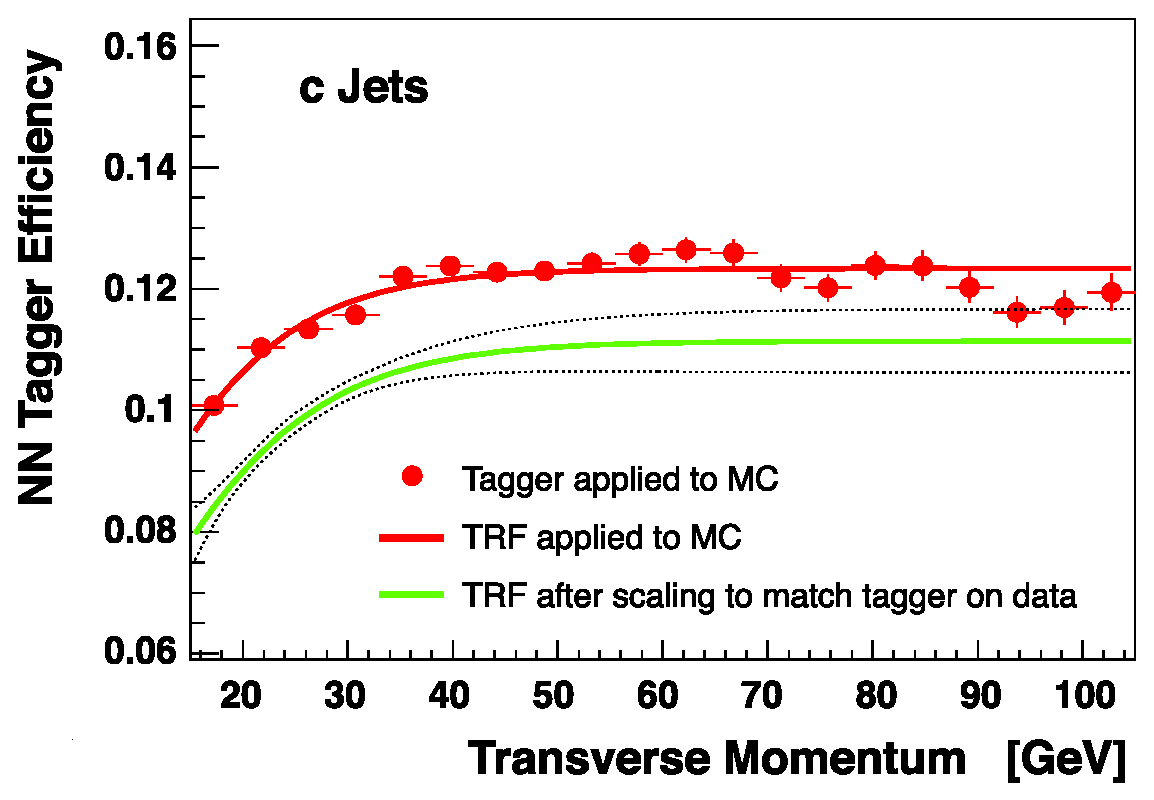
\includegraphics[width=0.32\textwidth]
{figures/TRF_c_pt.eps}
\hspace{0.6in}
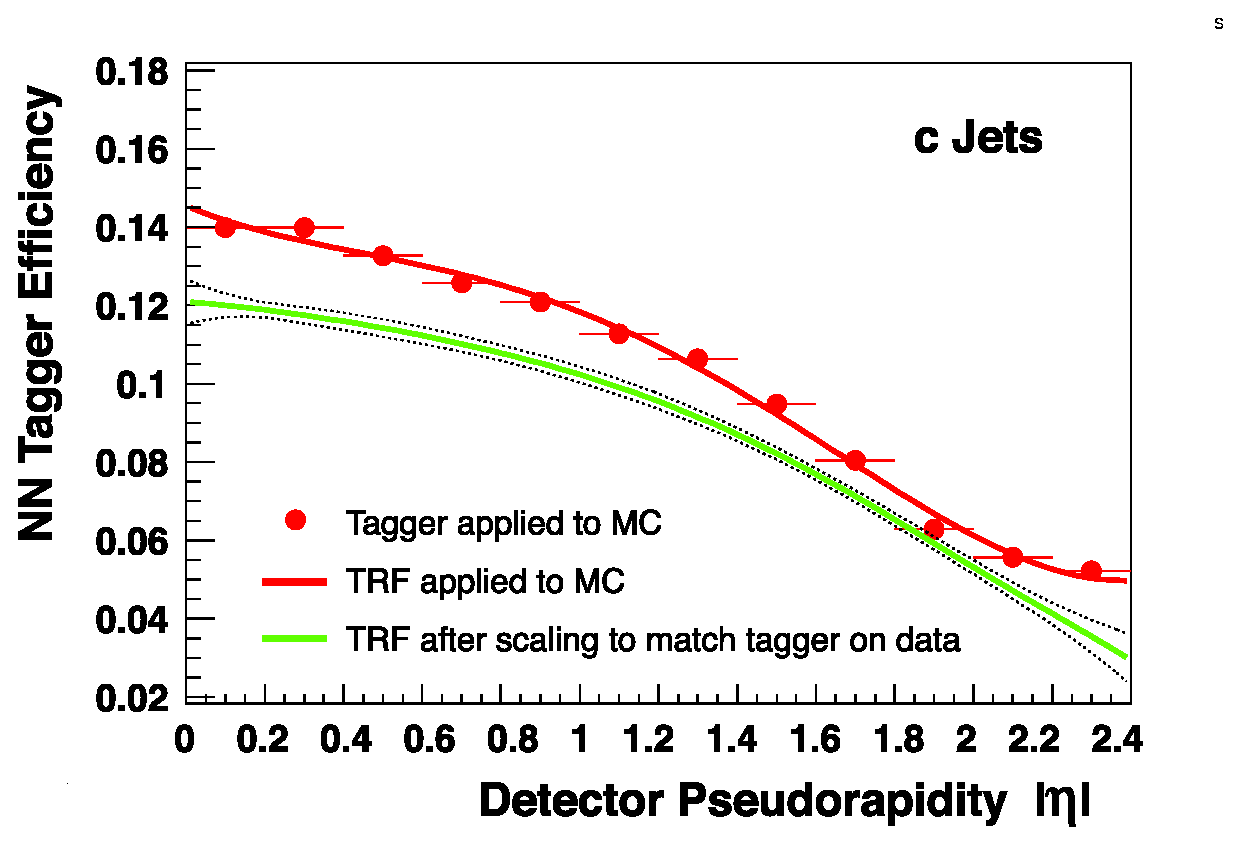
\includegraphics[width=0.35\textwidth]
{figures/TRF_c_eta.eps}
\vspace{-0.1in}
\begin{minipage}{5.5in}
\caption[nntagrf]{NN TIGHT tagger $b$-jet (upper row) and $c$-jet
(lower row) efficiencies as a function of $\pt$ (left column) and
$\eta$ (right column) in the inclusive $b$ and $c$ MC samples. The
corresponding data tag-rate functions ($\varepsilon_b$ and
$\varepsilon_c$) are also displayed.}
\label{fig:NNTRFs}
\end{minipage}
\end{figure}

\clearpage

The negative tag rate ($\varepsilon^{-}_{\rm data}$) measured in EM
and QCD data skims is used to estimate the fake, or mistag rate
$\varepsilon_{light}$. Each of the three taggers used as inputs for
the NN define a \emph{negative tag} differently: CSIP and JLIP as a
secondary vertex with negative impact parameter significance with
respect to the primary vertex, and SVT as a vertex with negative decay
length and $\Delta R<0.5$ with the jet. The NN tagger defines a
negative tag as the ouput from the NN when all three other taggers
yield a negative tag.

\vspace{0.1in}
The fake-tag rate $\varepsilon_{\rm light}$ is derived from the
negative tag rate, but needs to be corrected for the residual presence
of $b$- and $c$-quark jets in the negative tags and the asymmetry
between positive and negative tags. Two scale factors derived in MC
account for this:
\begin{eqnarray*}
\varepsilon_{\rm light}
& = & \varepsilon^{-}_{\rm data} \times SF_{hf} \times SF_{ll} \\
SF_{hf}
& = & \varepsilon^{-}_{\rm QCD~light}/\varepsilon^{-}_{\rm QCD~all} \\
SF_{ll}
& = & \varepsilon^{+}_{\rm QCD~light}/\varepsilon^{-}_{\rm QCD~light},
\end{eqnarray*}
where $SF_{hf}$ is the ratio between the number of negative tagged
jets from light quarks over the total number of negative tagged jets
in the QCD Monte Carlo. It is smaller than one if heavy-flavor jets
are present. And $SF_{ll}$ is the ratio between the number of positive
tagged jets from light quarks over the number of negative tagged jets
from light quarks in the QCD Monte Carlo. It is sensitive to
long-lived hadron decays in light-quark jets.


\subsection{$b$-Tagging Event Weights and $b$-Jet Assignment
Combinations}
\label{permuter}

Given the three different efficiencies $\varepsilon_{\alpha}$ outlined
above for $\alpha$ = $b$, $c$ and light jets, the probability to tag a
jet of flavor $\alpha$, or Tag Rate Function (TRF) can be expressed as
the product of the taggability and the tagging efficiency:
$$
\mathcal{P}_{\alpha}(\pt,\eta) = P^{\rm taggable}(\pt,\eta)\times \varepsilon_{\alpha}(\pt,\eta)
$$
Using the per jet probability, we can deduce the event probability
to contain zero, one or more than two tags:
\begin{eqnarray*}
P_{\rm event}(0~{\rm tag}) & = & \prod_{j=1}^{\rm N_{jets}}(1 - \mathcal{P}_{\alpha_j}(\pt_j,\eta_j)) \\
P_{\rm event}(1~{\rm tag}) & = & \sum_{j=1}^{\rm
N_{jets}}\mathcal{P}_{\alpha_j}(\pt_j,\eta_j) \prod_{i\neq j}(1 - \mathcal{P}_{\alpha_i}(\pt_i,\eta_i)) \\
P_{\rm event}(2~{\rm tags}) & = &
\sum_{j=1}^{\rm N_{jets}}\mathcal{P}_{\alpha_j}(\pt_j,\eta_j)
\prod_{i\neq j}\mathcal{P}_{\alpha_i}(\pt_i,\eta_i)
\prod_{k\neq j \neq i}(1 - \mathcal{P}_{\alpha_k}(\pt_k,\eta_k))
\end{eqnarray*}

By using TRFs we can estimate the number of tagged events, but this
does not help in knowing whether an individual jet is tagged or not,
since the TRF returns a weight. If one wants to use kinematic
variables using tagged or untagged jets, one needs to split each event
based on the number of jets and the number of possible tags and assign
for each permutation which jet or jets are tagged/untagged, with the
corresponding weight. Therefore each event is taken into account
several times, making sure that the sum of weights for all possible
combinations in each event returns the original probability for the
event to be not-tagged, tagged once or tagged twice.  This method
allows to use kinematic variables that rely on using $b$-tagging
information on the jets.
 